%%%%%%%%%%%%%%%%%%%%%%%%%%%%%%%%%%%%%%%%%%%%%%%%%%%%%%%%%%%%%%%%%%%%%%%%%%%%%%%%
%2345678901234567890123456789012345678901234567890123456789012345678901234567890
%        1         2         3         4         5         6         7         8
\documentclass[letterpaper, 10 pt, conference]{IEEEtran}
\IEEEoverridecommandlockouts
% The preceding line is only needed to identify funding in the first footnote. 
% If that is unneeded, please comment it out.
\usepackage{fancyhdr}   % Page number in header
\pagestyle{fancy}
\fancyhf{}
\fancyhead[R]{\thepage}
\usepackage{tabu,multirow}  % Thicker table lines
\usepackage{pifont}       % \ding
\newcommand{\xmark}{\ding{55}}
\usepackage{cite}
\usepackage{amsmath,amssymb,amsfonts}
\usepackage{algorithmic}
\usepackage{graphicx}
\usepackage{textcomp}
\usepackage[dvipsnames]{xcolor}
\def\BibTeX{{\rm B\kern-.05em{\sc i\kern-.025em b}\kern-.08em
    T\kern-.1667em\lower.7ex\hbox{E}\kern-.125emX}}
\makeatletter
\let\NAT@parse\undefined
\makeatother
\usepackage{hyperref}
\hypersetup{colorlinks,linkcolor={blue},citecolor={red},
            urlcolor={cyan},filecolor={magenta}}
%%%%%%%%%%%%%%%%%%%%%%%%%%%%%%%%%%%%%%%%%%%%%%%%%%%%%%%%%%%%%%%%%%%%%%%%%%%%%%%%
\begin{document}

\title{\LARGE \bf
Visual SLAM using ORB-SLAM2 with Path Finding*\\
\thanks{*This work was supported by Nvidia, XMotors.ai and UC Davis ECE 
        department.}
}

\author{Runlin Guo$^{1}$, Zhengfeng Lai$^{1}$ and Wenda Xu$^{1}$%
\thanks{$^{1}$The authors are all with the Electrical and Computer 
        Engineering Department at University of California - Davis, 
        1 Shields Ave, Davis, CA, USA. 
        {\tt\small \href{mailto:kolguo@ucdavis.edu}{kolguo@ucdavis.edu}, 
        \href{mailto:lzhengfeng@ucdavis.edu}{lzhengfeng@ucdavis.edu}, \newline 
        \href{mailto:wedxu@ucdavis.edu}{wedxu@ucdavis.edu}}}%
}

\maketitle
%%%%%%%%%%%%%%%%%%%%%%%%%%%%%%%%%%%%%%%%%%%%%%%%%%%%%%%%%%%%%%%%%%%%%%%%%%%%%%%%
\begin{abstract}
This paper presents a Visual SLAM approach, attempting to integrate ORB-SLAM2 
\cite{c1} system with path finding algorithm to achieve real-time autonomous 
navigation on a self-driving car. To diminish the disturbance of moving objects 
to camera pose estimation, we introduced a ORB feature refinement step using 
Mask R-CNN in the ORB-SLAM2 pipeline to remove the ORB features that belong to 
moving objects. For this purpose, we employed a Python-to-C++ code wrapper for 
ORB-SLAM2. We evaluated the Python wrapper and our feature refinement approach 
using the 11 sequences of KITTI dataset on a standard desktop computer. Our 
approach achieves mostly better performance compared to the original ORB-SLAM2 
system in pose estimation accuracy. We also attempted to integrate ORB-SLAM2 
system onto a radio controlled car using two RGB cameras and one Nvidia Jetson 
TX2 module. We performed an evaluation using KITTI dataset and compared the 
results with desktop performance. 
\end{abstract}

\begin{IEEEkeywords}
Visual odometry, Simultaneous localization and mapping, Real-time systems, 
Deep learning, Path planning
\end{IEEEkeywords}
%%%%%%%%%%%%%%%%%%%%%%%%%%%%%%%%%%%%%%%%%%%%%%%%%%%%%%%%%%%%%%%%%%%%%%%%%%%%%%%%
\section{Introduction} \label{sect:\thesection}
The Simultaneous Localization and Mapping (SLAM) problem is a computational 
problem of estimating the robot's poses and constructing the map of an unknown
environment at the same time. It is the basis for most autonomous navigation 
systems. Visual SLAM is a type of SLAM where the observation measurements are 
obtained mainly using camera sensors. Its advantages include
\begin{itemize}
    \item Cheap and easy to use camera sensors, contrast to LiDAR sensors.
    \item Not affected by wheel slip in uneven terrain, contract to classical 
    wheel odometry. 
\end{itemize}

Visual SLAM methods can be categorized into \textit{feature-based} or 
\textit{direct} based on tracking method and \textit{monocular}, 
\textit{stereo}, or \textit{RGB-D} based on type of camera sensors used.
\textit{Feature-based} visual SLAM methods add an additional step to extract 
and match feature points before tracking while \textit{direct} methods use 
the full image to track. A comparison of these two methods are summarized in 
Table \ref{tab:1}. 

\begin{table}[htbp]
\caption{Comparison of Feature-Based Method and Direct Method \cite{c2}}
\begin{center}
\begin{tabular}{|c|c|}
\hline
\textbf{Feature-Based} & \textbf{Direct}\\
\hline\hline 
\color{red}Can only use \& 
& \color{ForestGreen}Can use \& \\
\color{red}reconstruct corners 
& \color{ForestGreen}reconstruct whole image \\
\hline
\color{ForestGreen}Generally faster 
& \color{red}Generally slower \\

& \color{red}(but good for parallelism) \\
\hline
\color{ForestGreen}Flexible: outliers can be 
& \color{red}Inflexible: difficult to remove \\
\color{ForestGreen}removed retroactively 
& \color{red}outliers retroactively \\
\hline
\color{ForestGreen}Robust to inconsistencies in the
& \color{YellowOrange}Not robust to inconsistencies in \\
\color{ForestGreen}model/system (rolling shutter) 
& \color{YellowOrange}the model/system (rolling shutter) \\
\hline
\color{red}Decisions (KP detection) based 
& \color{ForestGreen}Decision (linearization point) based \\
\color{red}on less complete information 
& \color{ForestGreen}on more complete information \\
\hline
\color{ForestGreen}No need for good initialization 
& \color{YellowOrange}Needs good initialization \\
\hline
$\sim$20+ years of intensive research 
& $\sim$4 years of research \\
\hline
\end{tabular}
\label{tab:1}
\end{center}
\end{table}

To solve the problem, we used the state-of-the-art ORB-SLAM2 system. It has the
following advantages: 
\begin{itemize}
    \item Complete \textit{feature-based} visual SLAM system.
    \item Works with monocular, stereo and RGB-D camera sensors.
    \item Operates in real time on standard CPUs, in small and large, indoor
    and outdoor environments. 
    \item Allows wide baseline loop closing and relocalization.
    \item Includes full automatic initialization.
    \item Has excellent robustness and generates a compact and trackable map 
    that grows if the scene content changes, allowing life-long operation.
\end{itemize}
Therefore, ORB-SLAM achieves unprecedented performance with respect to other 
state-of-the-art visual SLAM approaches. This is the main motivation on 
investigating this specific algorithm. 

However, when generating the ORB features, the ORB-SLAM2 system does not 
differentiate between moving objects (such as cars and pedestrian) and 
stationary objects (such as roads and landmarks). Incorporating features 
belonging to moving objects into tracking misleads the system about camera 
translations and rotations. This reduces the accuracy of camera pose estimation.

Our goal is to implement a visual SLAM system based on ORB-SLAM2 and incorporate
an additional feature refinement step using Mask R-CNN. Also, we want to 
incorporate path finding algorithm to achieve auto navigation. In the end, we 
want to integrate ORB-SLAM2 system onto RC car using two cameras and a Nvidia 
Jetson TX2 module to test in real-world environment. 

Our feature refinement method is described in Section \ref{sect:III} and the 
path finding approach is described in Section \ref{sect:IV}. Our evaluation
methods and results are described in Section \ref{sect:V}. 

%%%%%%%%%%%%%%%%%%%%%%%%%%%%%%%%%%%%%%%%%%%%%%%%%%%%%%%%%%%%%%%%%%%%%%%%%%%%%%%%
\section{Related Work} \label{sect:\thesection}
\subsection{Monocular SLAM} \label{sect:\thesubsection}
Monocular SLAM was based on filter initially: every frame of video was processed
by the filter to calculate the map feature locations as well as camera pose. 
There exists a significant drawback in this methods: the computation over 
processing consecutive frames wastes a wealth of sources but gains little new
information over frames while also resulting in the huge accumulation of 
linearization errors. Later on, keyframe-based approaches use only selected 
frames. The famous system, PTAM by Klein and Murray \cite{c3}, successfully 
splits camera tracking and mapping in parallel threads for real time in small 
environments for the first time. But the points are only useful for tracking 
rather than for place recognition, making it hard operate in detecting large 
loops and yielding a low invariance to viewpoint.

Strasdat et. al \cite{c4} presented a large scale monocular SLAM system with a 
front-end based on optical flow implemented on a GPU, followed by FAST feature 
matching and motion-only BA, and a back-end based on sliding-window bundle 
adjustment (BA). 

Pirker et. al \cite{c5} proposed CD-SLAM, a very complete system including loop 
closing, relocalization, large scale operation and efforts to work on dynamic
environments.

The visual odometry of Song et. al \cite{c6} comes up ORB features for tracing 
and a temporal sliding window BA back-end. So it needs to reuse the map for 
global relocalization and loop detection, resulting delay for real-time 
detection. 

The semi-direct visual odometry SVO of Forster et. al \cite{c7} is a halfway 
between direct and feature based methods. Without requiring to extract features 
in every frame they are able to operate at high frame-rates obtaining impressive
results in quadcopters.

The recent work known as LSD-SLAM using monocular camera by Engel et. al
\cite{c8} can set up large-scale semi-dense maps based on direct methods rather
than bundle adjustment over features, This system is able to work out in real 
time and construct a semi-dense map but without GPU acceleration. However, the 
accuracy of camera localization seems relatively low and it still requires 
features for loop detection. Later, a version of LSD-SLAM using stereo cameras
\cite{c9} also appeared.

\subsection{Stereo and RGB-D SLAM} \label{sect:\thesubsection}
ORB-SLAM by Mur-Artal et. al \cite{c10} performs well in several aspects. It 
utilizes the same features for tracking, mapping, relocalization and loop 
closing simultaneously. So this system is highly efficient and reliable. And it
uses ORB features, which allow real-time operation without GPUs, for real time 
operation in large environments, such as loop closing based on the optimization
of a pose graph, camera relocalization and mapping points. Later, the ORB-SLAM2
using monocular, stereo and RGB-D cameras \cite{c1} also appeared.

The Computer Vision Group of the Technical University of Munich also develops a
Visual-SLAM algorithm named Direct Sparse Odometry (DSO) \cite{c11}. DSO is a
novel direct and sparse formulation for Visual Odometry and does not depend on
keypoint detectors or descriptors. It combines a fully direct probabilistic
model (minimizing a photometric error) with consistent, joint optimization of
all model parameters, including geometry - represented as inverse depth in a
reference frame - and camera motion. This is achieved in real time by omitting
the smoothness prior used in other direct methods and instead sampling pixels
evenly throughout the images. Since then, more variants of the DSO-SLAM method
have been published: Stereo DSO \cite{c12} in which stereo cameras are used,
Visual-Inertial DSO \cite{c13} in which an inertial measurement unit (IMU) is
used, DSO with Loop Closure (LSDO) \cite{c14} and Deep Virtual Stereo Odometry
(DVSO) \cite{c15} in which a deep monocular depth prediction using a novel deep
neural network is performed to overcome limitations of geometry-based monocular
visual odometry.

%%%%%%%%%%%%%%%%%%%%%%%%%%%%%%%%%%%%%%%%%%%%%%%%%%%%%%%%%%%%%%%%%%%%%%%%%%%%%%%%
\section{Mask R-CNN Feature Refinement} \label{sect:\thesection}
\begin{center}\textbf{Zhengfeng Lai, Runlin Guo}\end{center}

In this section, we are going to apply Mask R-CNN to the original ORB-SLAM2
system for solving the ``relative motion'' challenge. Since the open-sourced
ORB-SLAM2 system is in C++11, to apply Mask R-CNN in Python, we need a Python
wrapper for ORB-SLAM2 system. The Python wrapper is described in Section
\ref{sect:III-A} and the actual feature refinement approach is described in
Section \ref{sect:III-B}. 

\subsection{Python Wrapper Overview} \label{sect:\thesubsection}
We integrated the Python wrapper for ORB-SLAM2 system by John Skinner
\cite{python} into our system environment. The Python wrapper uses
\textit{Boost.Python} library which enables seamless interoperability between
C++ and Python and supports
\begin{itemize}
    \item Automatic cross-module type conversions
    \item Efficient function overloading
    \item Manipulating Python objects in C++
    \item Exporting C++ iterators as Python iterators
\end{itemize}

The execution flow of our system with the Python wrapper is as follows: 
\begin{itemize}
    \item Python wrapper loads stereo images using \\
    \texttt{opencv2.imread()}.
    \item The wrapper passes the stereo images to C++11.
    \item Tracking timestamps are measured and recorded in the Python wrapper.
    \item The wrapper gets camera poses trajectory from C++11 for evaluation.
\end{itemize}

The evaluation of this Python wrapper is provided in Section \ref{sect:V-B}. 

\subsection{Feature Refinement} \label{sect:\thesubsection}
Imaging the car is waiting on an intersection but there are several moving
objects around the car, ORB-SLAM2 system will simulate this case and generate
the results that the car is moving while obviously the car is waiting there,
which is called ``relative motion''. In order to diminish the disturbance of
moving objects to camera pose estimation, we designed an ORB feature refinement
step using Mask R-CNN in the ORB-SLAM2 pipeline to abandon the ORB features
that belong to moving objects. 

In the tracking thread, the ORB-SLAM2 system is going to extract the feature
points among every frame. However, considering the effect of ``relative 
motion'', the feature points extracted from moving contents definitely have
negative effect on the tracking thread because these points may lead the system
to make wrong estimations on camera estimation and lower the accuracy. Hence our
group decided to remove these points, which means we are saving useful feature
points for tracking rather than those negative-effect points. 

In order to get these points, we applied Mask R-CNN to segment every moving
content of each frame of the video. After this step, we can get the area which
has moving contents, as Fig. \ref{fig:1}. After using Mask R-CNN, we can obtain
the segmentation of all objects in the frame. The following step is to find the
areas of moving contents. Obviously during driving, the moving contents around
the car can only be pedestrians, cars and bicycles. So we set the label that if
the objects detected by Mask R-CNN are in the above categories, the objects are
moving contents. And we will abandon all feature points in these moving areas,
which indicates that once the extracted feature points by tracking thread are
in these areas, we will remove them out for the following threads. 

\begin{figure}[ht]
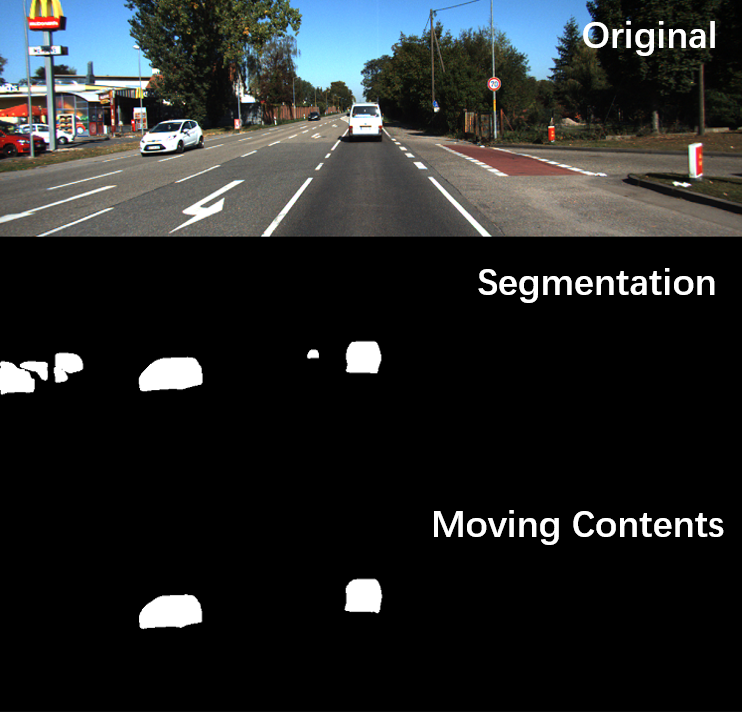
\includegraphics[scale=0.7]{images/maskrcnnrm.png}
\caption{Remove Moving Contents}
\label{fig:1}
\end{figure}

The evaluation of our feature refinement approach is provided in Section
\ref{sect:V-C}.

%%%%%%%%%%%%%%%%%%%%%%%%%%%%%%%%%%%%%%%%%%%%%%%%%%%%%%%%%%%%%%%%%%%%%%%%%%%%%%%%
\section{Path Finding} \label{sect:\thesection}
\begin{center}\textbf{Wenda Xu}\end{center}

In this section, we did researches on several popular path finding algorithms
and tried to find an optimal cost function specifically applied to Visual SLAM. 

\subsection{Main Algorithm comparisons:} \label{sect:\thesubsection}
Dijkstra, greedy first search and A* algorithm are three main techniques, which
are commonly used for path finding. Dijkstra's algorithm works by repeatedly
examines the closet not-yet-examined vertex, adding its vertices to the set of
vertices to be examined. Based on the nature of this algorithm, it is guaranteed
to find the shortest path with all the positive edges. However, its speed is not
optimized. The Greedy Best-First-Search algorithm on the contrary has the
heuristic of how far from the goal any vertex is. Instead of selecting the
vertex closet to the starting point, it selects the vertex closet to the goal.
Greedy-Best-First search is not guaranteed to find a shortest path, but it is
much quicker compared to Dijkstra's Algorithm because of its heuristic function.
In the end, A* Algorithm uses both the exact cost of the path from the starting
point to any vertex n, and heuristic estimated cost from vertex n to the goal to
represent cost function. Therefore, based on the nature and better performance
of A* algorithm, we use A* algorithm as our baseline model to further
investigate on optimizing its cost function corresponding to Visual SLAM
application. 

\subsection{Goal and Algorithm intuitions:} \label{sect:\thesubsection}
Our goal is trying to minimize the reconstruction uncertainty of observed
geometry and the distance traveled by the sensor between image locations.
However, specific visual SLAM challenge is lack of ground truth data. we need to
evaluate the statistical uncertainty in order to estimate reconstruction quality
\cite{c18} (Gaussian distribution of the data points). Based on referencing
paper ``\textit{Optimal View Path Planning for Visual SLAM}'', we have the
intuition (Greedy approach: Solve a local minimal problem to global
minimal) \cite{c18} and specific algorithm (Levenberg-Marquardt method) to
develop cost function. General idea is to evaluate cost function before any
observations are made and to predict the camera view at a particular location
based on the current data distribution.

\subsection{Specific algorithm works as follows:} \label{sect:\thesubsection}
The following descriptions of the algorithm is obtained from the paper
``\textit{Optimal View Path Planning for Visual SLAM}'' \cite{c18}.

Step1: Given initial data points distribution, calculate centroid and assign
this to be the interest point of camera. Select a target location for the
camera, i.e, select the end point of the path.

Step2: Use linear interpolation to generate a initial path between the first and
last camera locations. Use the image sampling rate and speed of the robot camera
to verify results.

Step3: Find a minimum of the cost function using LM (Levenberg-Marquardt)
method.

Step4: Move the camera to the next location along the path and make an actual
observation. Update the camera interest point and path end point. 

Repeat Step 3 and Step 4, each time with one less camera location, update the
initial guess using the previous path estimation. In the end, a single path will
be converged and the algorithm will obtain the minimum distance between
optimized image locations.

\subsection{Proposed cost function:} \label{sect:\thesubsection}

\begin{equation}\begin{split}
C(P,X) &= \frac{1}{N} \times tr(\sum_{} P,X) + \frac{\alpha}{(M - 1)^{1 - q}}\\
&\sum_{j=1}^{M-1}||P_{pos}^{j+1} - P_{pos}^{j}||^q + \beta H(n)^*
\label{eq}
\end{split}\end{equation}

The first two terms came from the proposed cost function\cite{c18} from paper
``\textit{Optimal View Path Planning for Visual SLAM}'', the later term H(n) is
the heuristic function came from the A* algorithm, which measures the cost from
vertex n to the goal. Beta and alpha are parameters required to tune for both
functions. The first term measures the camera position path along the path
within the estimated data points distributions. Original paper proposed to use
functions of the eigenvalues of co-variance matrix to solve condensing
probability distribution problem. Since eigenvalues have a direct geometric
interpretation \cite{c18}, the eigenvalues of each block can correspond to the
variance of the feature location, calculating the trace of co-variance of matrix
to minimize the sum of the eigenvalues. In another words, it minimizes the total
reconstructed uncertainty of converging to the optimal path. 

\noindent\fbox{\begin{minipage}[t]{0.47\textwidth}
\begin{center}\end{center}
\begin{center}\textbf{Difficulties and Future Notice}\end{center} 

\begin{enumerate}
    \item Key difficulty is to tune the hyper parameters Alpha and Beta
    \cite{c18}. Alpha is the weight which controls camera path between data
    points. If Alpha is setting too high, the path will be less easy to
    modified, optimal path will be away from the data points. The first term,
    will increase as uncertainty of each data point increases. If alpha value
    was set too low, path will tend to get closer to the data points. In that
    case, uncertainty of each data points can get dramatically decreased.
    However, the overall path is deviated a lot. Therefore, Alpha is important 
    in determine path shape and minimizing total costs. At the same time, Beta
    is also an important factor. If Beta was set too high, then algorithm will
    not guaranteed to find a shortest path but speed is fast. On the contrary,
    if Beta is too small, algorithm is guaranteed to find the shortest path.
    However, more nodes will be expanded and make the running time much slower.
    \item The other difficulty is to cop-orate with Visual-SLAM based map
    points. Using data points alone from the Visual SLAM can't cover the entire
    data point that we needed, such as some data points of the obstacles. We
    need to develop a more comprehensive methods to collect all the data points
    that needed in path finding.
\end{enumerate}
\end{minipage}}

%%%%%%%%%%%%%%%%%%%%%%%%%%%%%%%%%%%%%%%%%%%%%%%%%%%%%%%%%%%%%%%%%%%%%%%%%%%%%%%%
\section{Evaluation} \label{sect:\thesection}
\begin{center}\textbf{Runlin Guo, Zhengfeng Lai}\end{center}

We have evaluated the original ORB-SLAM2 system, the Python wrapper, our feature
refinement approach and the ORB-SLAM2 system on Jetson TX2 using the 11
sequences of KITTI dataset \cite{c17} with ground truth poses. There are three
evaluating metrics: 
\begin{itemize}
    \item $tran$ - Average relative camera pose translation (movement) error
    [\%]
    \item $rot$ - Average relative camera pose rotation error \newline
    [degree/100m]
    \item $time$ - Average tracking time [second]
\end{itemize}
The camera pose translation error and rotation error will determine the accuracy
of the SLAM system while the tracking time will determine whether the system can
achieve real-time tracking performance. 

Our evaluation is performed on a desktop computer with an Intel Core i7-7820X,
an NVIDIA GeForce GTX 1080 Ti and 32 GB of system RAM.

\subsection{Original ORB-SLAM2 C++11 System} \label{sect:\thesubsection}
The evaluation results below are the average results obtained by running 10
iterations of the 11 sequences of KITTI dataset.
\begin{itemize}
    \item Translation Error: \newline
    A boxplot of the translation error is shown in Fig. \ref{fig:CTrans}. As we
    can see, sequence 01 has relatively significant translation error. This is
    because it is the only highway sequence among the 11 sequences. Therefore,
    there are few close trackable points, making it harder to estimate camera
    translation. A frame with colored trackable points from sequence 01 is shown
    in Fig. \ref{fig:KITTI01}. 
    
    \begin{figure}[htbp]
    \centerline{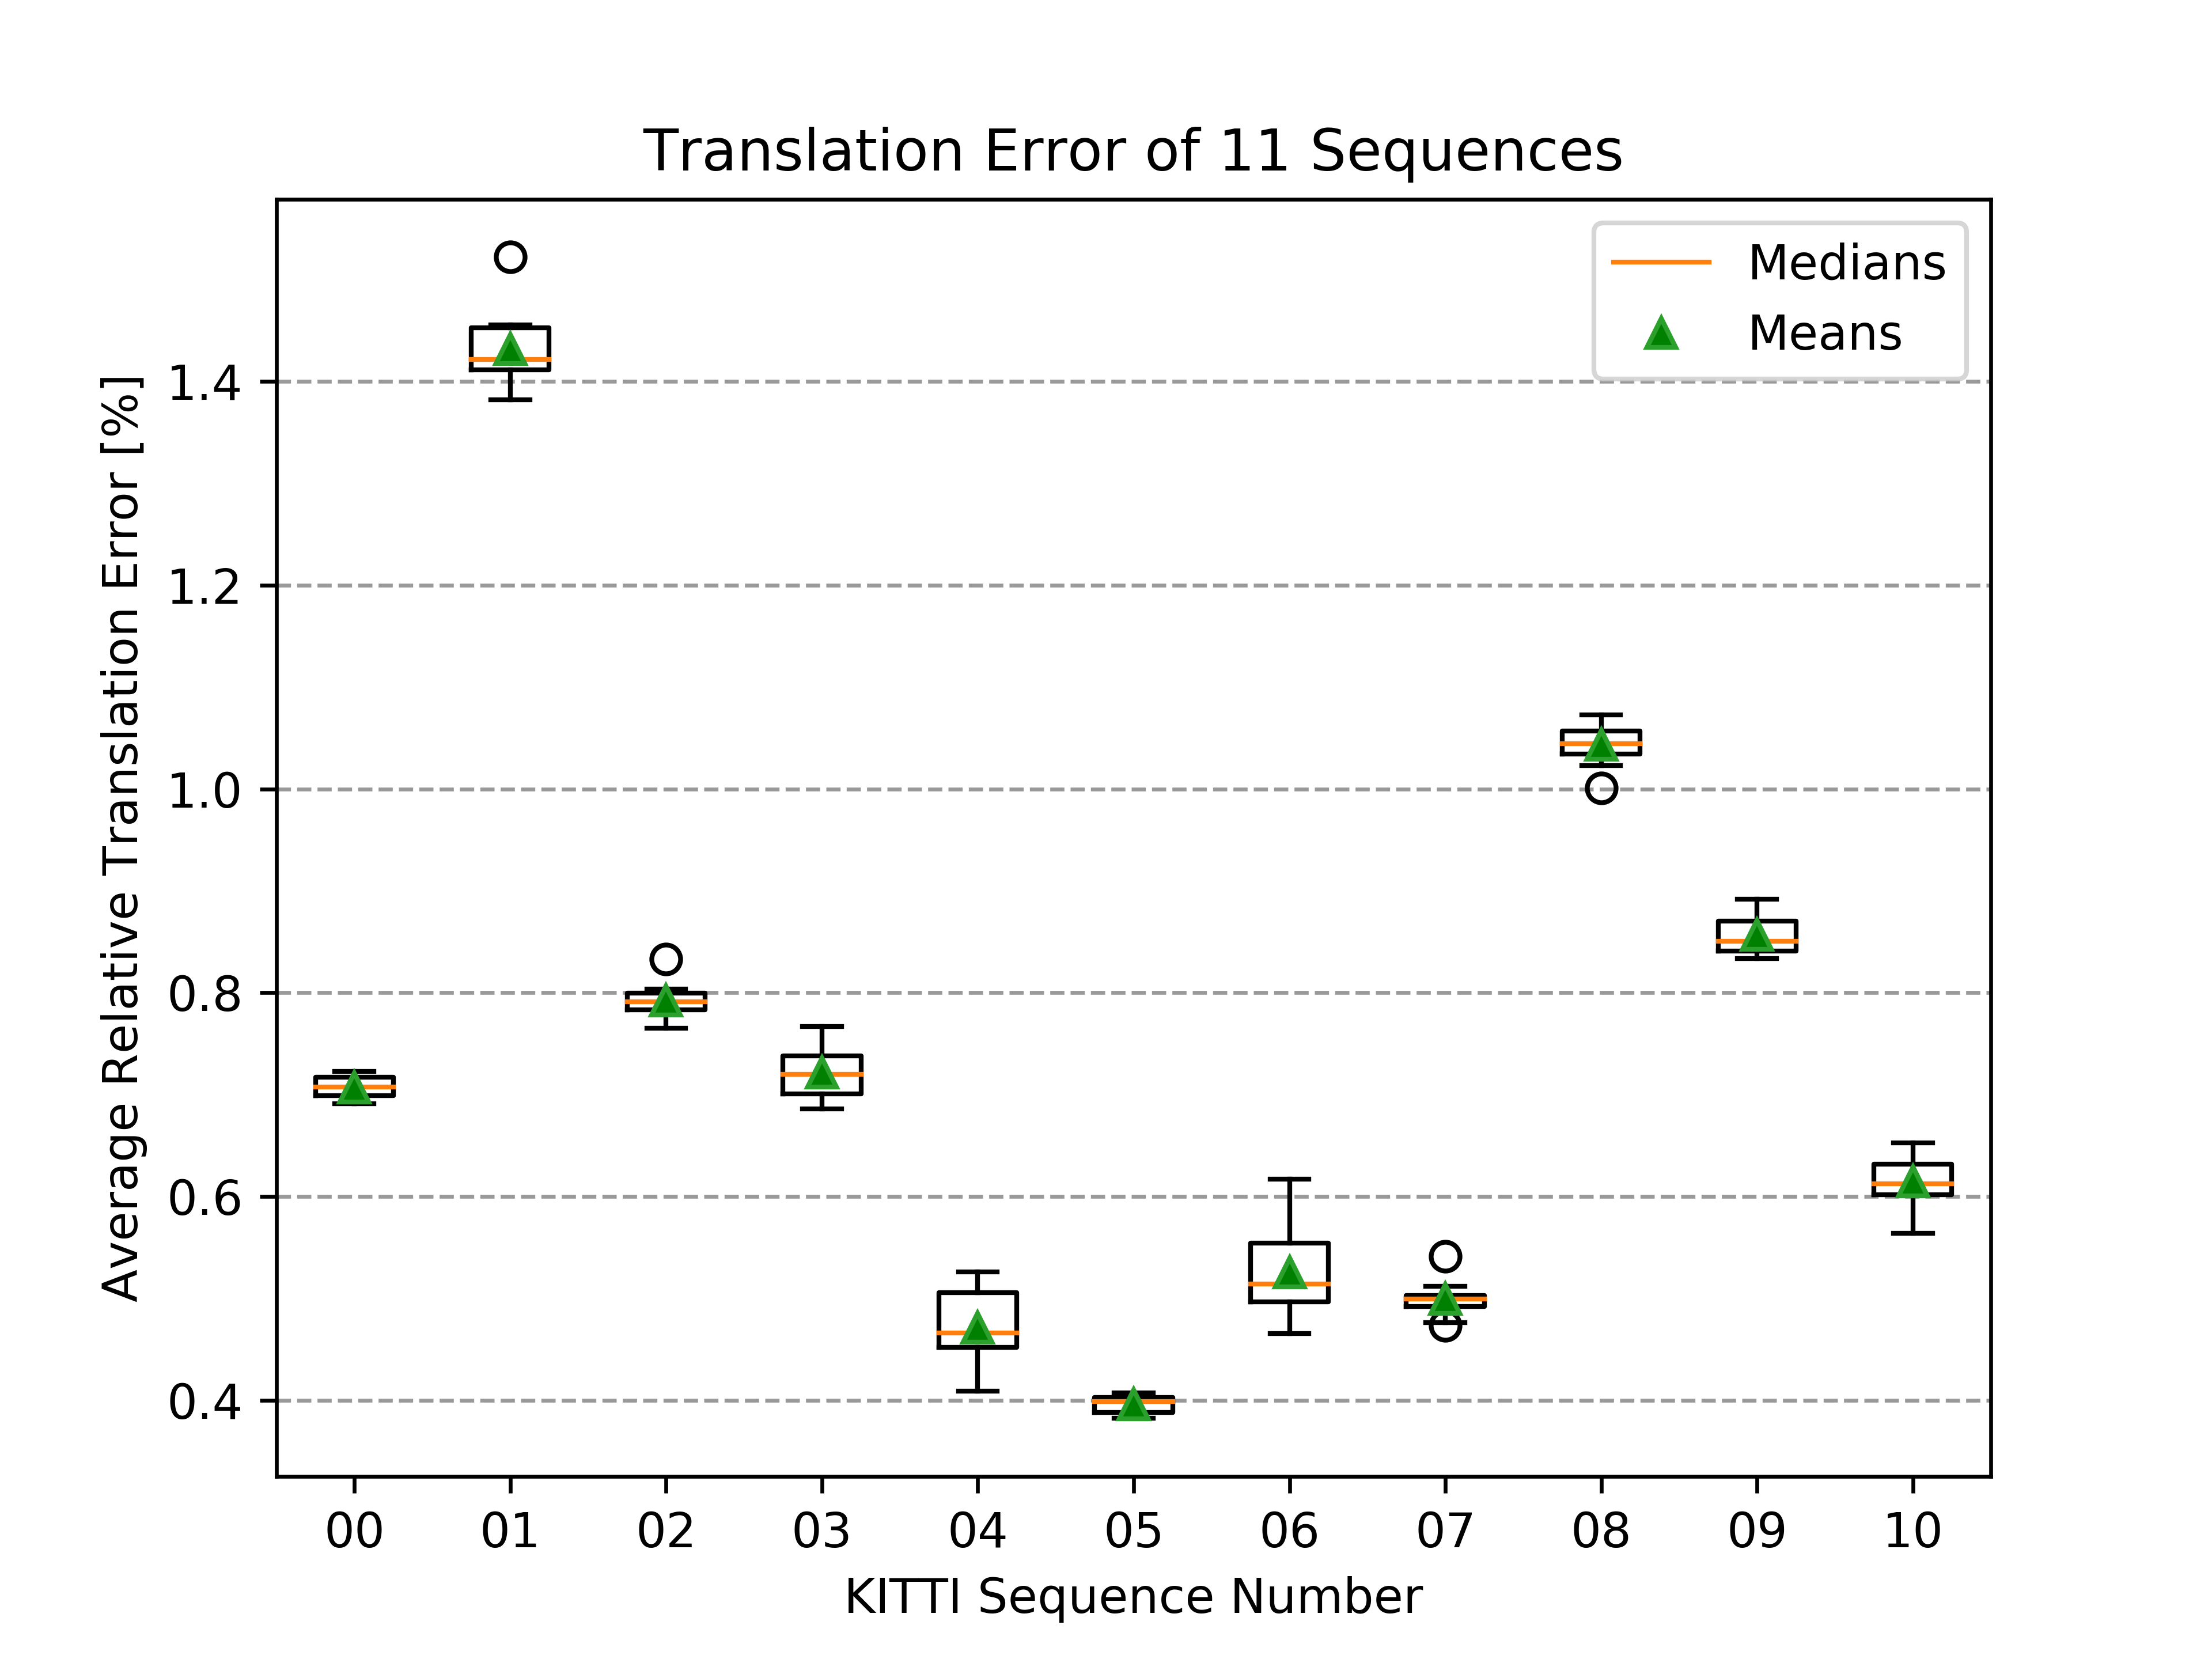
\includegraphics[scale=0.59]
    {images/Evaluation/C++/trans_error.png}}
    \caption{C++11 Translation Error}
    \label{fig:CTrans}
    \end{figure}
    
    \begin{figure}[htbp]
    \centerline{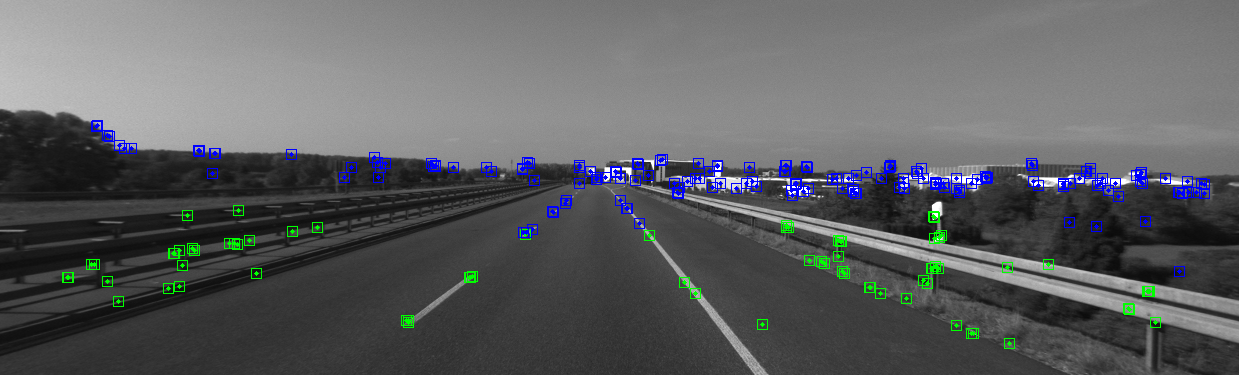
\includegraphics[scale=0.2]
    {images/Evaluation/C++/Sequence_01_Tracked_Points.png}}
    \caption{Tracked Points in KITTI Sequence 01. Green points are close
    trackable points while blue points are far trackable points.}
    \label{fig:KITTI01}
    \end{figure}
    
    \item Rotation Error: \newline
    A boxplot of the rotation error is shown in Fig. \ref{fig:CRot}. As we
    can see, sequence 08 has relatively significant rotation error. This is
    because it has repeated paths which do not form loops, plenty of sharp turns
    and few distant trackable points, making it harder to estimate camera
    rotation. The trajectory of this sequence is shown in Fig.
    \ref{fig:KITTI08}. 
    
    \begin{figure}[htbp]
    \centerline{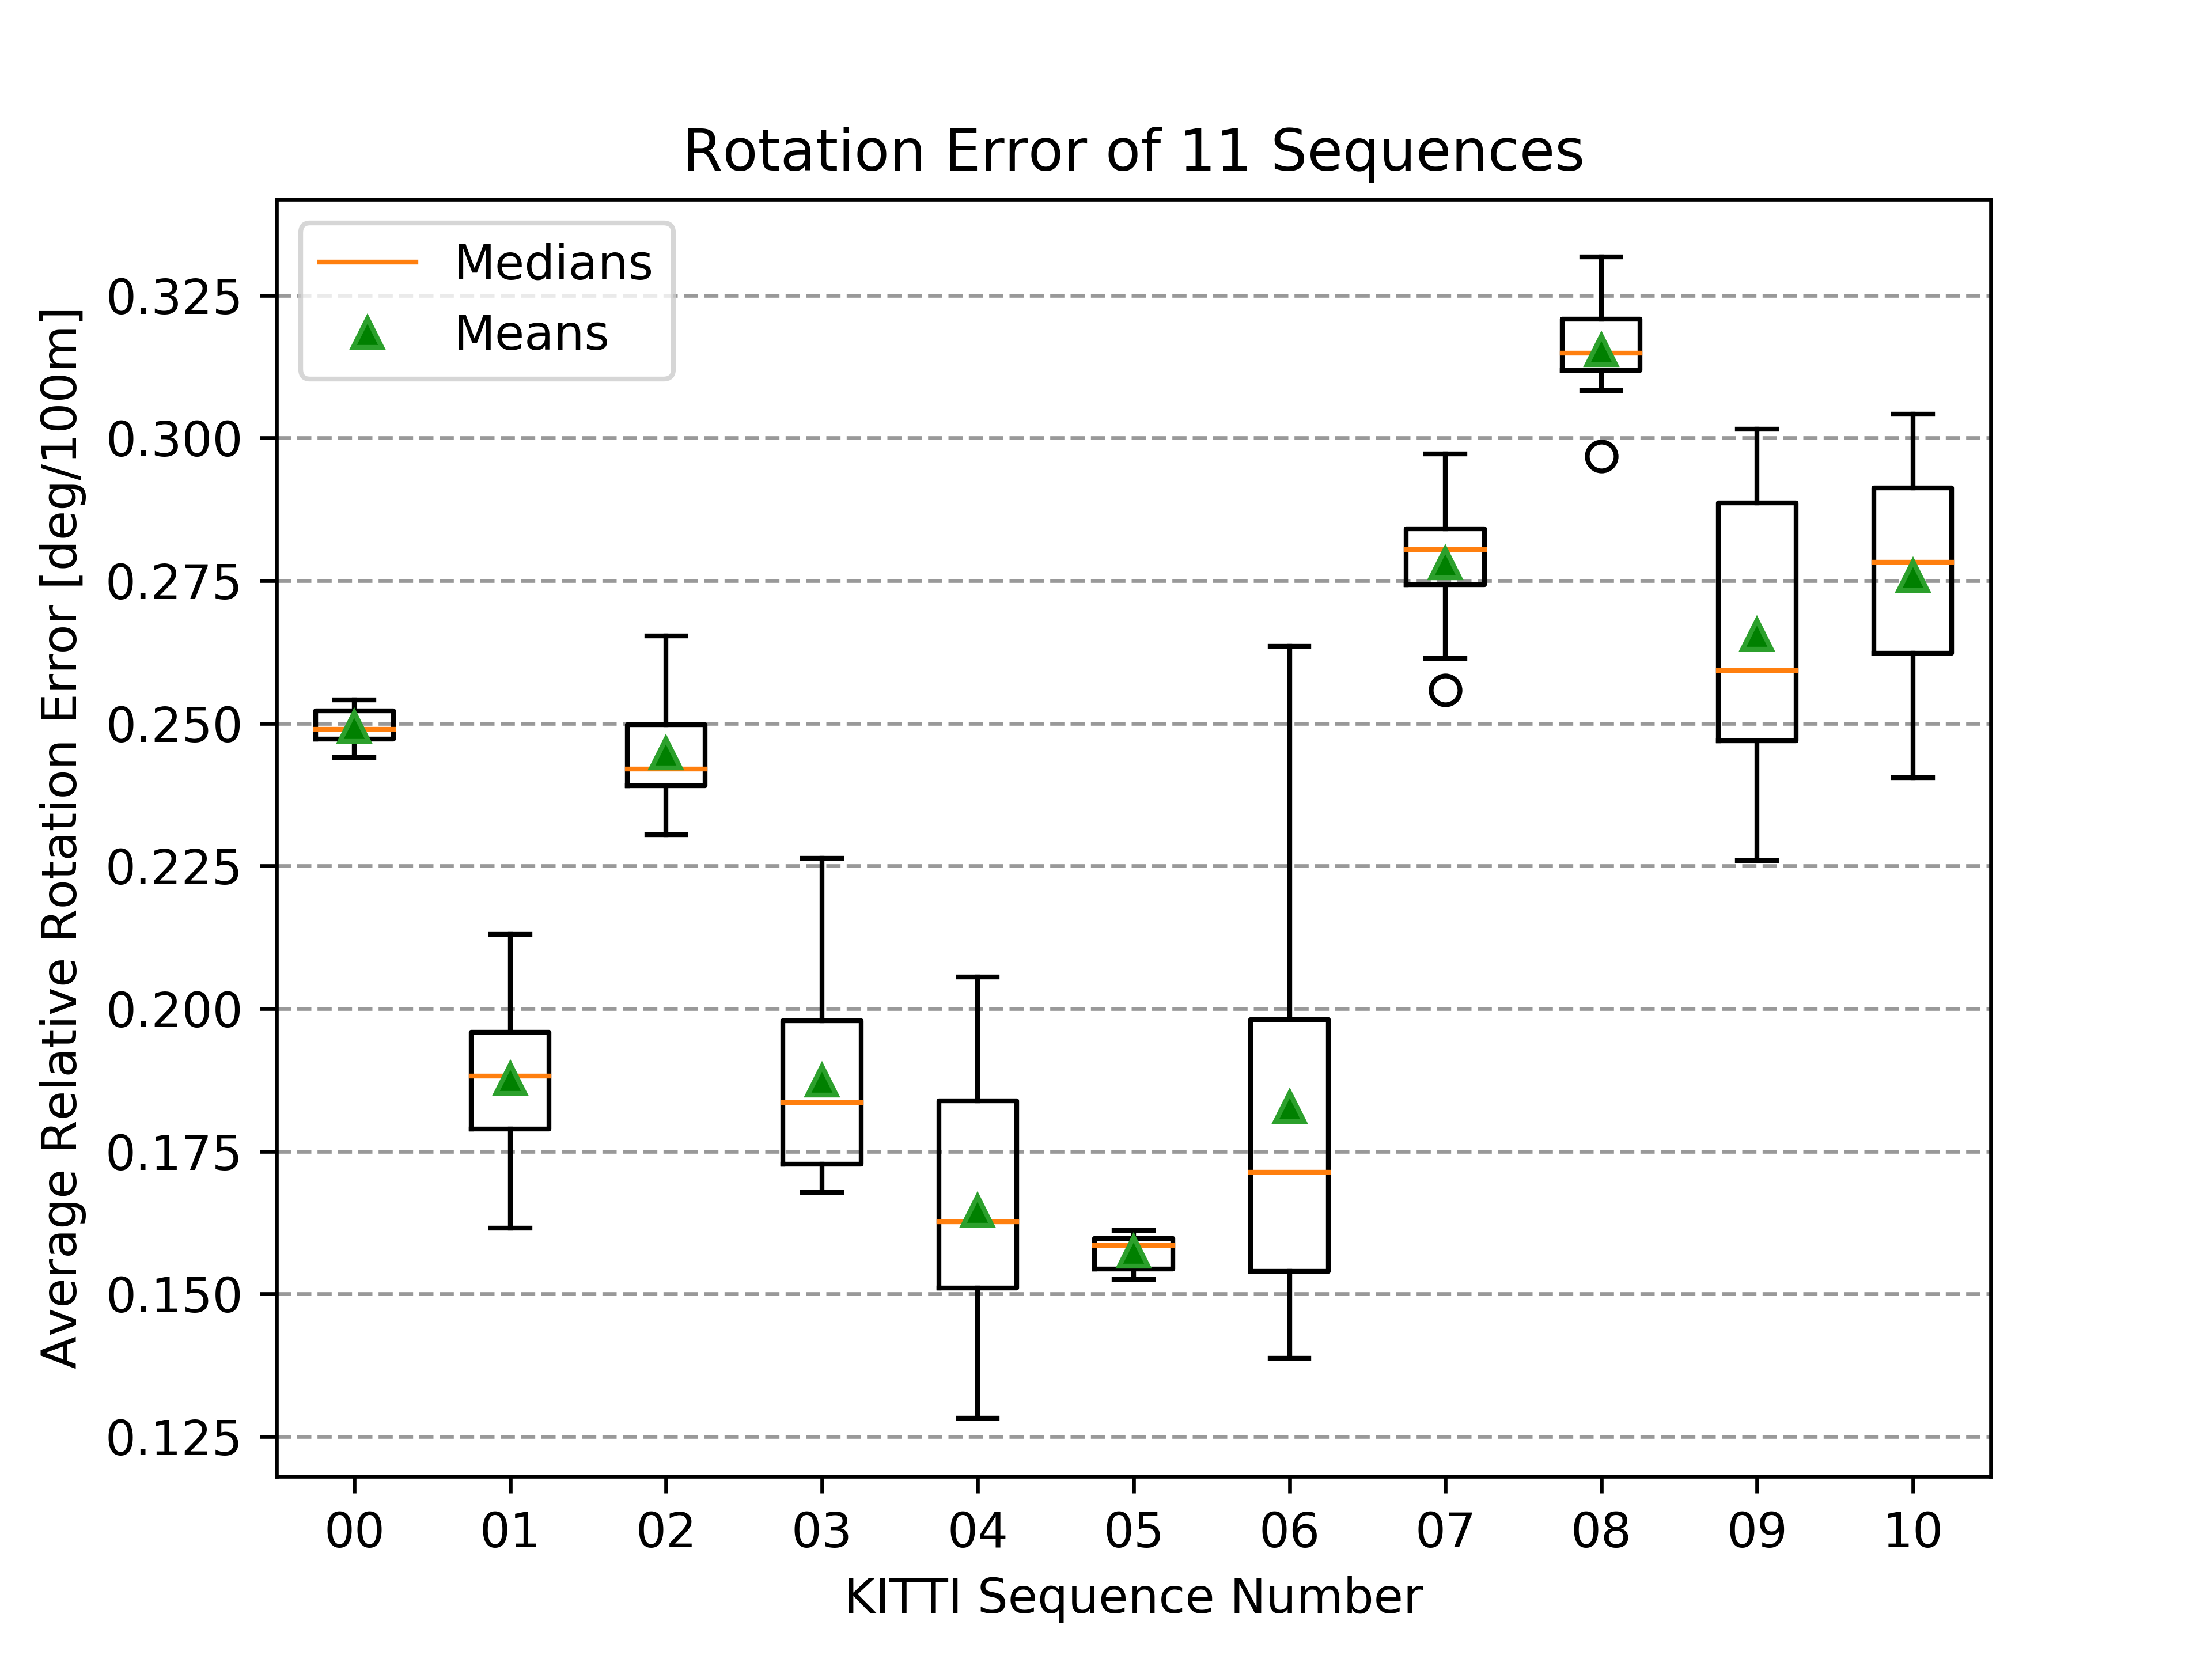
\includegraphics[scale=0.59]
    {images/Evaluation/C++/rot_error.png}}
    \caption{C++11 Rotation Error}
    \label{fig:CRot}
    \end{figure}
    
    \begin{figure}[htbp]
    \centerline{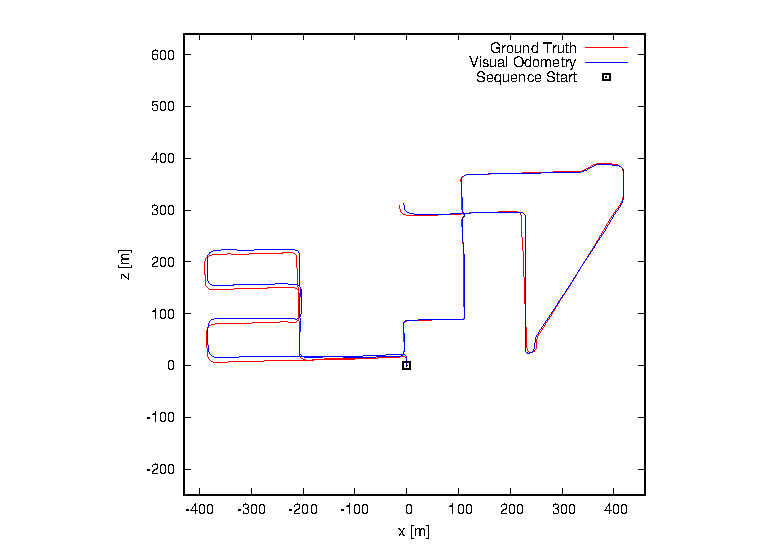
\includegraphics[scale=1]
    {images/Evaluation/C++/Sequence_08_path.eps}}
    \caption{Trajectory Path of KITTI Sequence 08. Red path is ground truth
    trajectory while blue path is the estimated trajectory.}
    \label{fig:KITTI08}
    \end{figure}

    \item Mean Tracking Time: \newline
    A boxplot of the mean tracking time is shown in Fig. \ref{fig:CTime}. As we
    can see, sequence 01 has relatively significant mean tracking time. This is
    because in this highway sequence, the car is moving at high speed and the
    camera captures at low frame rate (only 10 fps). Therefore, it is important
    to insert keyframes often enough so that the amount of close points allows
    for accurate translation estimation and no tracking lost occurs. The
    increased frequency of keyframe insertion requires more computing power,
    resulting in longer tracking time. 
    
    Also, since the camera frame rate is 10 Hz, the frame time is
    $\frac{1}{10}=0.1$ second. Because all 11 sequences result in less mean
    tracking time than 0.1 second, the system is operating in real-time. 
    
    \begin{figure}[htbp]
    \centerline{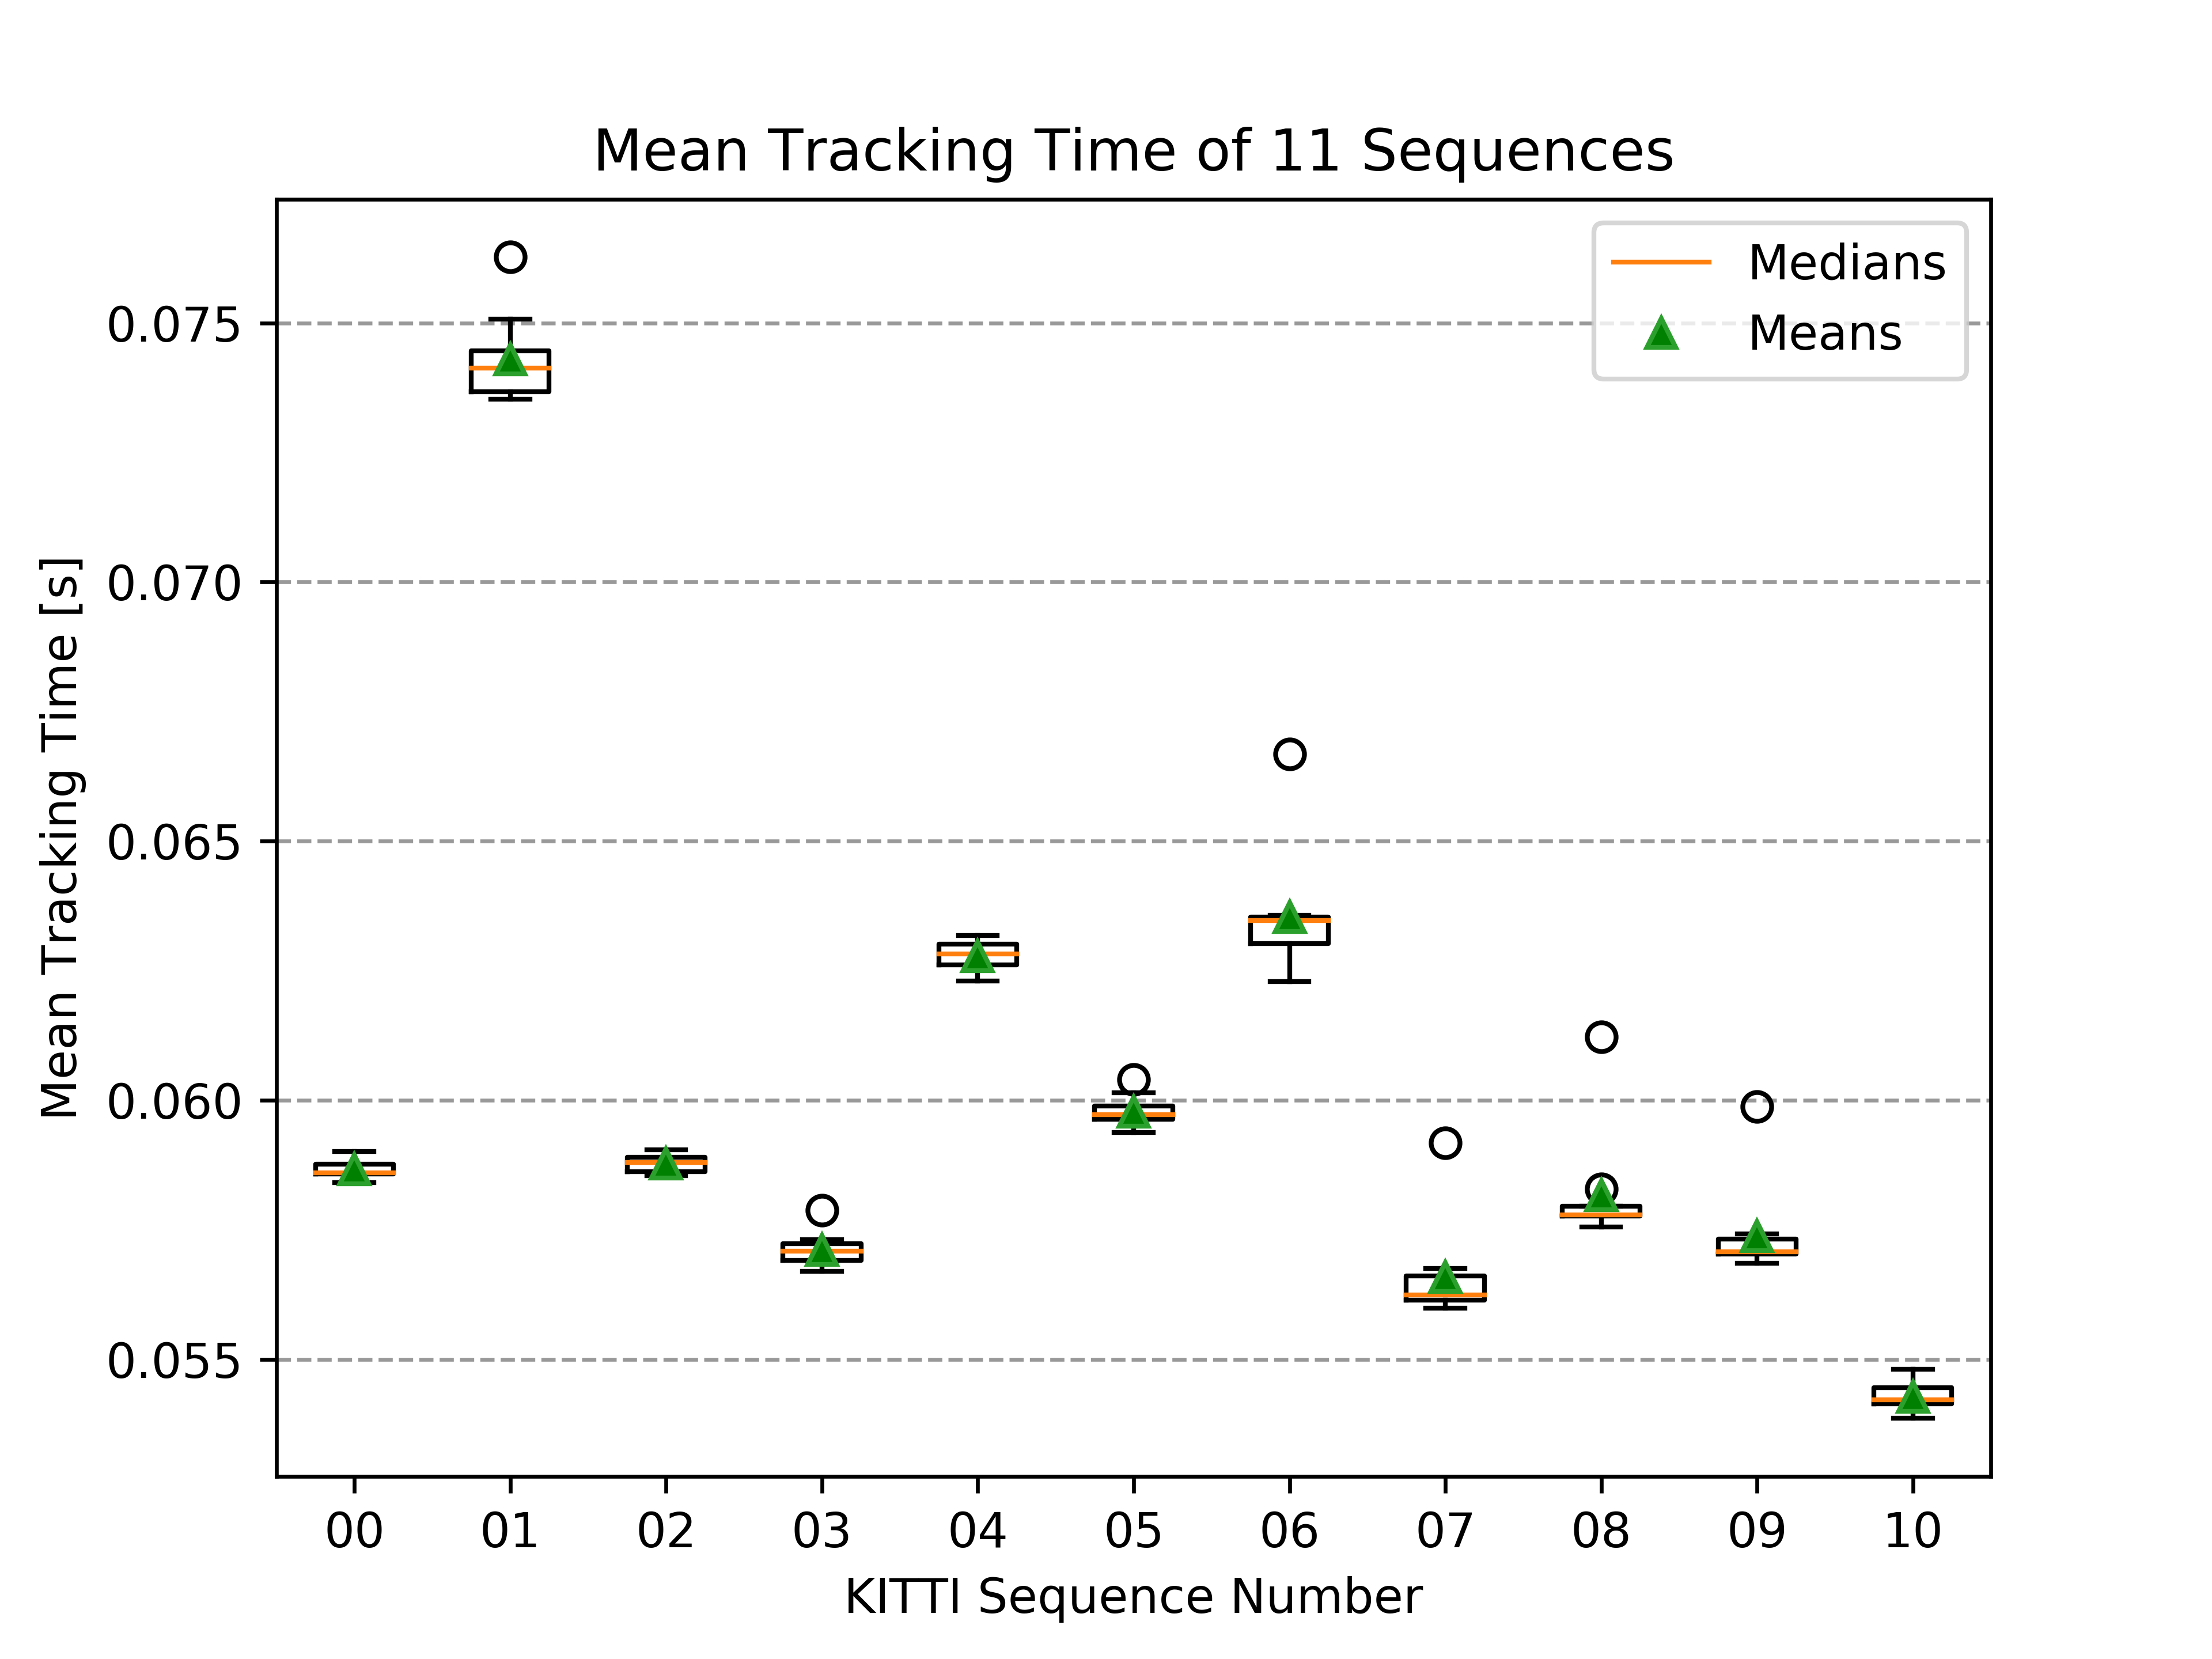
\includegraphics[scale=0.59]
    {images/Evaluation/C++/mean_track_time.png}}
    \caption{C++11 Mean Tracking Time}
    \label{fig:CTime}
    \end{figure}
\end{itemize}

\begin{figure}[htbp]
\centerline{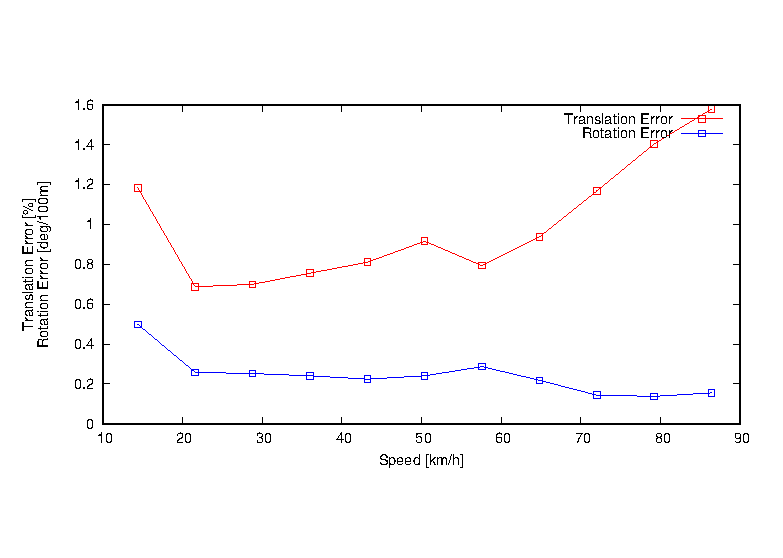
\includegraphics[width=9cm, height=8cm]
{images/Evaluation/C++/Avg_speed_tranroterr.eps}}
\caption{Average Translation and Rotation Error vs. Speed}
\label{fig:AvgSpeed}
\end{figure}

In summary, we concluded that the ORB-SLAM2 system
\begin{itemize}
    \item Generates \textbf{larger translation error} under \textbf{high speed
    and low frame rate}. This can be further illustrated by Fig.
    \ref{fig:AvgSpeed} which is a plot of translation and rotation error versus
    speed. As we can see, the translation error increases rapidly when the speed
    exceeds 60 km/h. 
    \item Generates \textbf{larger translation error} with \textbf{few close}
    trackable points.
    \item Generates \textbf{larger rotation error} with \textbf{few distant}
    trackable points.
\end{itemize}

\subsection{Python Wrapper} \label{sect:\thesubsection}
The evaluation results below are the average results obtained by running 10
iterations of the 11 sequences of KITTI dataset. The results are summarized in
Table \ref{tab:pyC}.
\begin{itemize} 
    \item Translation Error: \newline
    As we can see from the $trans$ column, the C++11 and Python wrapper have
    comparable translation error. If we look at the average result, the Python
    wrapper even performs slightly better: smaller mean and standard deviation. 
    
    \item Rotation Error: \newline
    As we can see from the $rot$ column, the C++11 and Python wrapper have
    comparable rotation error. If we look at the average result, the results of
    Python wrapper have smaller standard deviation. 
    
    Particularly, if we look at the highway sequence 01, the Python wrapper has
    much worse mean error: 0.226 compared to only 0.188 of C++11 system. Thus,
    the Python wrapper seems to suffer more under high speed and low frame rate
    situation. 

    \item Mean Tracking Time: \newline
    As we can see from the $time$ column, the Python wrapper has generally
    longer tracking time. This is probably due to the Python library overhead. 
\end{itemize}

\begin{table}[htbp]
\caption{Python Wrapper vs. C++11}
\begin{center}
\begin{tabu}{|c||c|c|c|c|c|c|}
\hline
\textbf{Sequence}&\multicolumn{2}{c|}{\textbf{$trans\>[\%]$}} &
\multicolumn{2}{c|}{\textbf{$rot\>[deg/100m]$}} &
\multicolumn{2}{c|}{\textbf{$time\>[sec]$}}\\
\cline{2-7} 
\textbf{\#} & \textbf{\textit{Mean}}& \textbf{\textit{Std dev}}&
\textbf{\textit{Mean}}& \textbf{\textit{Std dev}}& \textbf{\textit{Mean}}&
\textbf{\textit{Std dev}} \\
[-1pt] \tabucline[1pt]{1-7}
00 C++ & \color{ForestGreen}0.707 & 0.011 & \color{ForestGreen}0.249 &
\color{ForestGreen}0.003 & \color{ForestGreen}0.059 & 
\color{ForestGreen}0.0002 \\
\hline
00 Py & 0.708 & \color{ForestGreen}0.010 & 0.254 & 0.007 & 0.060 & 0.0005 \\
\hline\hline
01 C++ & 1.432 & 0.038 & \color{ForestGreen}0.188 & \color{ForestGreen}0.017 &
\color{ForestGreen}0.074 & \color{ForestGreen}0.0008 \\
\hline
01 Py & \color{ForestGreen}1.409 & \color{ForestGreen}0.027 & 0.226 & 0.018 &
0.075 & 0.0011 \\
\hline\hline
02 C++ & 0.792 & \color{ForestGreen}0.018 & 0.245 & 0.009 &
\color{ForestGreen}0.059 & \color{ForestGreen}0.0002 \\
\hline
02 Py & \color{ForestGreen}0.773 & 0.019 & \color{ForestGreen}0.241 &
\color{ForestGreen}0.007 & 0.060 & 0.0005 \\
\hline\hline
03 C++ & 0.721 & \color{ForestGreen}0.024 & 0.187 & 0.018 &
\color{ForestGreen}0.057 & \color{ForestGreen}0.0003 \\
\hline
03 Py & \color{ForestGreen}0.719 & 0.027 & \color{ForestGreen}0.174 &
\color{ForestGreen}0.012 & 0.058 & 0.0004 \\
\hline\hline
04 C++ & 0.471 & 0.037 & 0.165 & 0.024 & \color{ForestGreen}0.063 &
\color{ForestGreen}0.0003 \\
\hline
04 Py & \color{ForestGreen}0.462 & \color{ForestGreen}0.030 &
\color{ForestGreen}0.159 & \color{ForestGreen}0.022 & 0.064 & 0.0006 \\
\hline\hline
05 C++ & \color{ForestGreen}0.396 & \color{ForestGreen}0.009 &
\color{ForestGreen}0.157 & \color{ForestGreen}0.003 & \color{ForestGreen}0.060
& \color{ForestGreen}0.0003 \\
\hline
05 Py & 0.409 & 0.018 & 0.165 & 0.008 & 0.061 & 0.0005 \\
\hline\hline
06 C++ & \color{ForestGreen}0.525 & 0.043 & 0.183 & 0.037 &
\color{ForestGreen}0.064 & 0.0011 \\
\hline
06 Py & 0.533 & \color{ForestGreen}0.018 & \color{ForestGreen}0.173 &
\color{ForestGreen}0.018 & 0.064 & \color{ForestGreen}0.0006 \\
\hline\hline
07 C++ & \color{ForestGreen}0.500 & \color{ForestGreen}0.018 &
\color{ForestGreen}0.278 & \color{ForestGreen}0.011 & \color{ForestGreen}0.057
& 0.0009 \\
\hline
07 Py & 0.518 & 0.059 & 0.283 & 0.023 & 0.057 & \color{ForestGreen}0.0005 \\
\hline\hline
08 C++ & 1.043 & 0.020 & 0.315 & 0.009 & \color{ForestGreen}0.058 & 0.0010 \\
\hline
08 Py & \color{ForestGreen}1.031 & \color{ForestGreen}0.018 &
\color{ForestGreen}0.307 & \color{ForestGreen}0.005 & 0.059 &
\color{ForestGreen}0.0005 \\
\hline\hline
09 C++ & 0.857 & \color{ForestGreen}0.018 & 0.266 & 0.024 &
\color{ForestGreen}0.057 & 0.0009 \\
\hline
09 Py & \color{ForestGreen}0.842 & 0.027 & \color{ForestGreen}0.240 &
\color{ForestGreen}0.013 & 0.058 & \color{ForestGreen}0.0005 \\
\hline\hline
10 C++ & \color{ForestGreen}0.615 & \color{ForestGreen}0.024 &
\color{ForestGreen}0.276 & \color{ForestGreen}0.019 & \color{ForestGreen}0.054
& \color{ForestGreen}0.0003 \\
\hline
10 Py & 0.617 & 0.027 & 0.282 & 0.026 & 0.055 & 0.0005 \\
[-1pt] \tabucline[1pt]{1-7}
Avg C++ & 0.733 & 0.287 & 0.228 & 0.055 & \color{ForestGreen}0.060 & 0.0052 \\
\hline
Avg Py & \color{ForestGreen}0.729 & \color{ForestGreen}0.277 & 0.228 &
\color{ForestGreen}0.053 & 0.061 & \color{ForestGreen}0.0051 \\
\hline
\end{tabu}
\label{tab:pyC}
\end{center}
\end{table}

In summary, compared with the C++11 system, we concluded that the Python wrapper
has
\begin{itemize}
    \item Almost the same translation error.
    \item Generally smaller variances but comparable means in rotation error. 
    \begin{itemize}
        \item Under high speed and low frame rate, Python wrapper performs
        worse.
    \end{itemize}
    \item Generally longer tracking time. 
\end{itemize}

Overall, there is not much influence on tracking accuracy by integrating the
Python wrapper. Therefore, it can be used to apply Mask R-CNN for feature
refinement. 

\subsection{Mask R-CNN Feature Refinement} \label{sect:\thesubsection}
Firstly, we ran our model on sequence 09 of KITTI dataset, and the result is
shown as Fig. \ref{fig:2}. The green line denotes the ORB-SLAM2 system with Mask
R-CNN while the red line denotes the original ORB-SLAM2 without Mask R-CNN. The
$x$-axis indicates the length that car has covered while the $y$-axis indicates
the translation error. According to Fig. \ref{fig:2}, we can find that generally
the system with Mask R-CNN has lower translation error, denoting it has better
achievements especially when the car has run over 300 meters. After 300 meters,
the translation error is considerably reduced. 
\begin{figure}[ht]
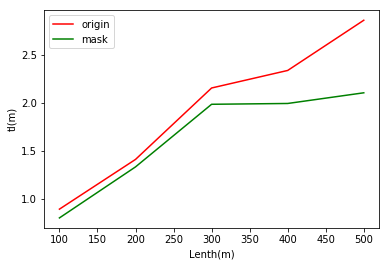
\includegraphics[scale=0.85]{images/Evaluation/FeatureRefine/compare.png}
\caption{With VS. Without Mask R-CNN}
\label{fig:2}
\end{figure}

Later on, we also tested the 11 sequences of KITTI dataset. The performance of
the original ORB-SLAM2 and Mask R-CNN combined model is shown in Fig.
\ref{fig:3}. We can obtain the fact that ORB-SLAM2 with Mask R-CNN in most
sequences achieves lower error in both rotation and movement error. 
\begin{figure}[ht]
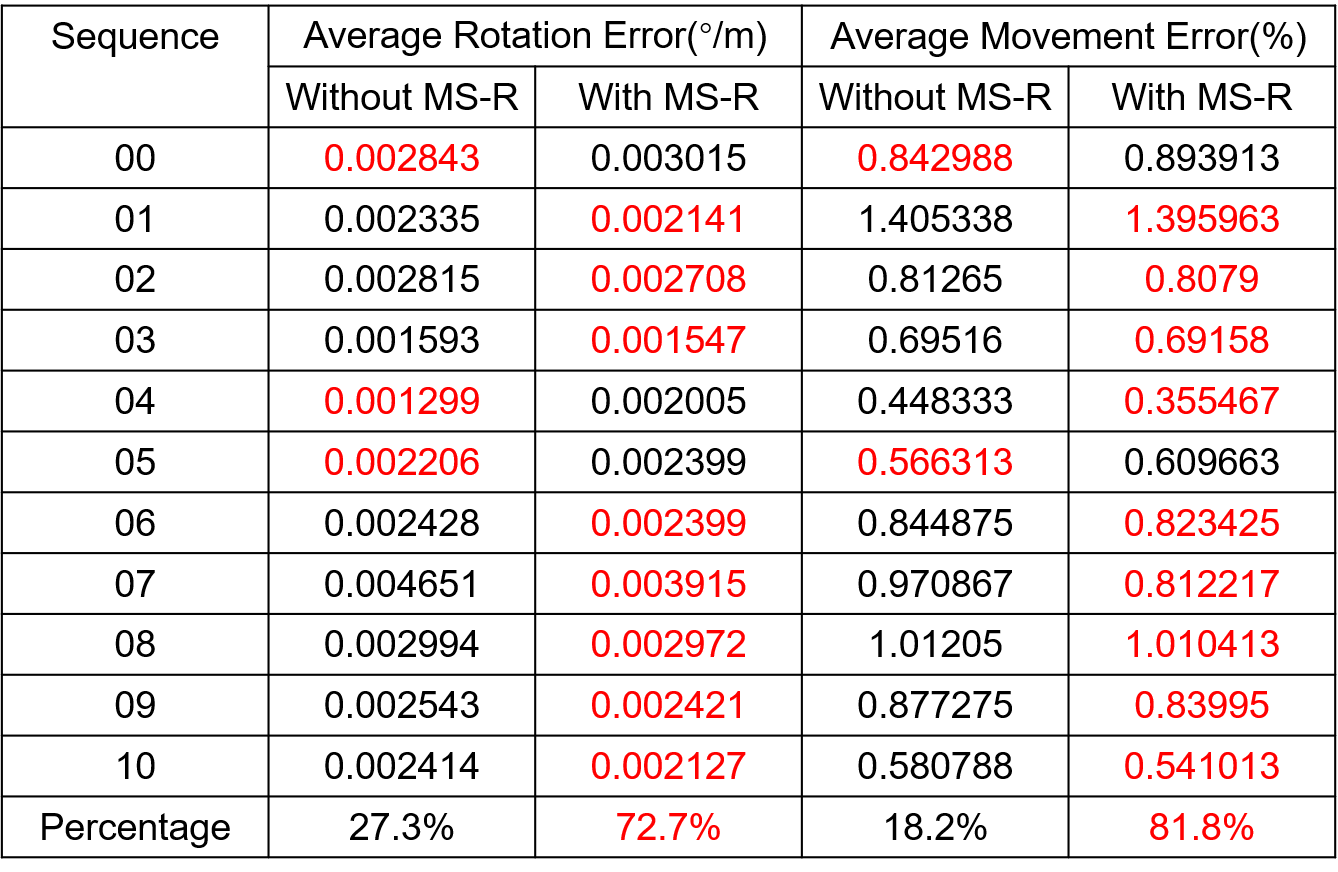
\includegraphics[scale=0.39]{images/Evaluation/FeatureRefine/versus.png}
\caption{Performance on KITTI Sequence}
\label{fig:3}
\end{figure}

After calculating the exact performance, we can get the results as Fig.
\ref{fig:4}. It is obvious that with Mask R-CNN, the system could achieve lower
error and higher accuracy in both movement and rotation error. 
\begin{figure}[ht]
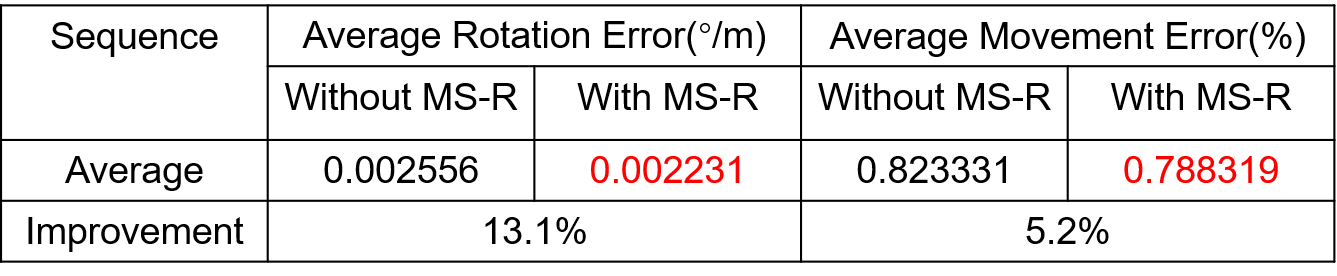
\includegraphics[scale=0.39]{images/Evaluation/FeatureRefine/versus2.png}
\caption{Improvement of ORB SLAM2 with Mask R-CNN}
\label{fig:4}
\end{figure}

\begin{figure}[htbp]
\centering
\begin{minipage}[t]{0.48\textwidth}
\centering
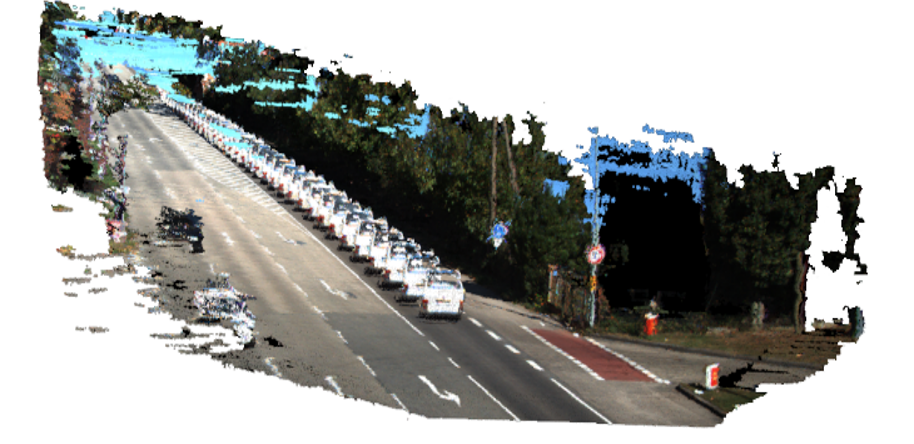
\includegraphics[width=6cm]
{images/Evaluation/FeatureRefine/Mappingwithoutmaskrcnn.png}
\caption{Mapping without Mask R-CNN}
\label{fig:5}
\end{minipage}
\begin{minipage}[t]{0.48\textwidth}
\centering
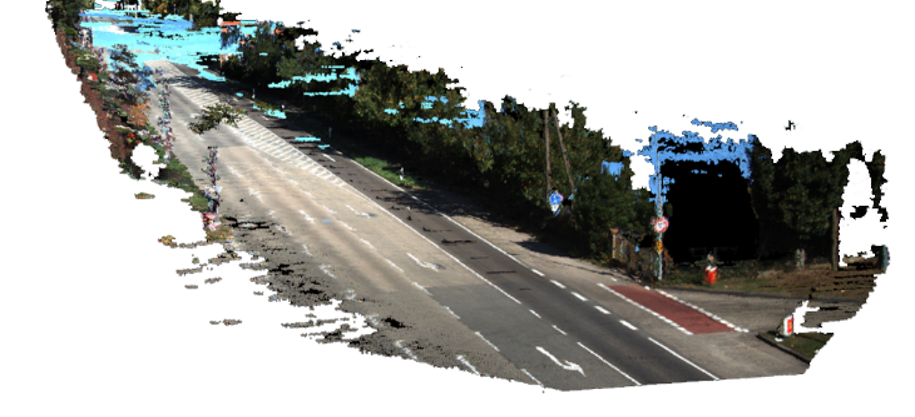
\includegraphics[width=6cm]
{images/Evaluation/FeatureRefine/mappingwithmaskrcnn.png}
\caption{Mapping with Mask R-CNN}
\label{fig:6}
\end{minipage}
\end{figure}

For the mapping thread, due to the limited time, we only tested one sequence of
KIITI dataset. And Fig. \ref{fig:5} and Fig. \ref{fig:6} visually and clearly
show the differnt performance of ORB SLAM2 with and without Mask R-CNN. If we
only use ORB-SLAM2 and all feature points extracted from moving contents are
used for tracking thread, we can see that there are many shadows of moving cars
in Fig. \ref{fig:5}. And obviously the generated map is not ideal and not that
clear. However, after using Mask R-CNN to move out the feature points from
moving contents, the generated map is much clearer with higher quality. 

\subsection{ORB-SLAM2 on Jetson TX2} \label{sect:\thesubsection}
The NVIDIA Jetson TX2 module has 6 ARM64v8 CPU cores, 8 GB of system RAM, 32 GB
of flash storage and a NVIDIA Pascal architecture GPU. After we installed the
environment onto Jetson TX2 and solved several library conflicts, we are able to
get the original ORB-SLAM2 system working. However, two of the KITTI dataset
sequences failed to run on the Jetson due to RAM shortage. Table
\ref{tab:jetson} shows some details about the 11 KITTI dataset sequences. The
evaluation results in Table \ref{tab:jetsonPy} are the average results obtained
by running 10 iterations of the 11 sequences of KITTI dataset. 

\begin{table}[htbp]
\caption{Details of KITTI Dataset Sequences$^{\mathrm{*}}$}
\begin{center}
\begin{tabular}{|c|c|c|}
\hline
\textbf{Sequence \#} & \textbf{\# of Frames} & \textbf{\# of Loops} \\
\hline\hline
\color{red}00 & \color{red}4541 & \color{red}4 \\
\hline
\color{ForestGreen}01 & \color{ForestGreen}1101 & \color{ForestGreen}0 \\
\hline
\color{red}02 & \color{red}4661 & \color{red}2 \\
\hline
\color{ForestGreen}03 & \color{ForestGreen}801 & \color{ForestGreen}0 \\
\hline
\color{ForestGreen}04 & \color{ForestGreen}271 & \color{ForestGreen}0 \\
\hline
\color{ForestGreen}05 & \color{ForestGreen}2761 & \color{ForestGreen}3 \\
\hline
\color{ForestGreen}06 & \color{ForestGreen}1101 & \color{ForestGreen}1 \\
\hline
\color{ForestGreen}07 & \color{ForestGreen}1101 & \color{ForestGreen}1 \\
\hline
\color{ForestGreen}08 & \color{ForestGreen}4071 & \color{ForestGreen}0 \\
\hline
\color{ForestGreen}09 & \color{ForestGreen}1591 & \color{ForestGreen}0 \\
\hline
\color{ForestGreen}10 & \color{ForestGreen}1201 & \color{ForestGreen}0 \\
\hline
\multicolumn{3}{l}{$^{\mathrm{*}}${\color{red}Red: Failed to run}, {\color{ForestGreen}Green: Succeeded to run}}
\end{tabular}
\label{tab:jetson}
\end{center}
\end{table}

\begin{table}[htbp]
\caption{Python ORB-SLAM2 Jetson TX2 vs. Desktop}
\begin{center}
\begin{tabu}{|c||c|c|c|c|c|c|}
\hline
\textbf{Sequence}&\multicolumn{2}{c|}{\textbf{$trans\>[\%]$}} &
\multicolumn{2}{c|}{\textbf{$rot\>[deg/100m]$}} &
\multicolumn{2}{c|}{\textbf{$time\>[sec]$}}\\
\cline{2-7} 
\textbf{\#} & \textbf{\textit{Mean}}& \textbf{\textit{Std dev}}&
\textbf{\textit{Mean}}& \textbf{\textit{Std dev}}& \textbf{\textit{Mean}}&
\textbf{\textit{Std dev}} \\
[-1pt] \tabucline[1pt]{1-7}
00 PC & \color{ForestGreen}0.708 & \color{ForestGreen}0.010 &
\color{ForestGreen}0.254 & \color{ForestGreen}0.007 & \color{ForestGreen}0.060 &
\color{ForestGreen}0.0005 \\
\hline
00 TX2 & \xmark & \xmark & \xmark & \xmark & \xmark & \xmark \\
\hline\hline
01 PC & \color{ForestGreen}1.409 & \color{ForestGreen}0.027 &
\color{ForestGreen}0.226 & \color{ForestGreen}0.018 & \color{ForestGreen}0.075 &
\color{ForestGreen}0.0011 \\
\hline
01 TX2 & 1.416 & 0.058 & 0.242 & 0.023 & 0.207 & 0.0021 \\
\hline\hline
02 PC & \color{ForestGreen}0.773 & \color{ForestGreen}0.019 &
\color{ForestGreen}0.241 & \color{ForestGreen}0.007 & \color{ForestGreen}0.060 &
\color{ForestGreen}0.0005 \\
\hline
02 TX2 & \xmark & \xmark & \xmark & \xmark & \xmark & \xmark \\
\hline\hline
03 PC & \color{ForestGreen}0.719 & \color{ForestGreen}0.027 &
\color{ForestGreen}0.174 & \color{ForestGreen}0.012 &\color{ForestGreen} 0.058 &
\color{ForestGreen}0.0004 \\
\hline
03 TX2 & 0.747 & 0.028 & 0.201 & 0.017 & 0.176 & 0.0008 \\
\hline\hline
04 PC & \color{ForestGreen}0.462 & \color{ForestGreen}0.030 &
\color{ForestGreen}0.159 & \color{ForestGreen}0.022 & \color{ForestGreen}0.064 &
0.0006 \\
\hline
04 TX2 & 0.479 & 0.038 & 0.215 & 0.036 & 0.194 & \color{ForestGreen}0.0005 \\
\hline\hline
05 PC & 0.409 & 0.018 & 0.165 & 0.008 & \color{ForestGreen}0.061 &
\color{ForestGreen}0.0005 \\
\hline
05 TX2 & \color{ForestGreen}0.395 & \color{ForestGreen}0.013 &
\color{ForestGreen}0.158 & \color{ForestGreen}0.005 & 0.191 & 0.0006 \\
\hline\hline
06 PC & 0.533 & \color{ForestGreen}0.018 & \color{ForestGreen}0.173 &
\color{ForestGreen}0.018 & \color{ForestGreen}0.064 & 
\color{ForestGreen}0.0006 \\
\hline
06 TX2 & \color{ForestGreen}0.491 & 0.040 & 0.175 & 0.032 & 0.194 & 0.0013 \\
\hline\hline
07 PC & 0.518 & 0.059 & 0.283 & 0.023 & \color{ForestGreen}0.057 & 0.0005 \\
\hline
07 TX2 & \color{ForestGreen}0.504 & \color{ForestGreen}0.028 & 0.283 &
\color{ForestGreen}0.015 & 0.183 & 0.0005 \\
\hline\hline
08 PC & \color{ForestGreen}1.031 & \color{ForestGreen}0.018 &
\color{ForestGreen}0.307 & \color{ForestGreen}0.005 & \color{ForestGreen}0.059 &
\color{ForestGreen}0.0005 \\
\hline
08 TX2 & 1.035 & 0.022 & 0.314 & 0.008 & 0.190 & 0.0009 \\
\hline\hline
09 PC & 0.842 & 0.027 & \color{ForestGreen}0.240 & 0.013 &
\color{ForestGreen}0.058 & \color{ForestGreen}0.0005 \\
\hline
09 TX2 & \color{ForestGreen}0.840 & \color{ForestGreen}0.026 & 0.248 &
\color{ForestGreen}0.011 & 0.186 & 0.0008 \\
\hline\hline
10 PC & 0.617 & 0.027 & 0.282 & 0.026 & \color{ForestGreen}0.055 &
\color{ForestGreen}0.0005 \\
\hline
10 TX2 & \color{ForestGreen}0.591 & \color{ForestGreen}0.016 &
\color{ForestGreen}0.275 & \color{ForestGreen}0.018 & 0.178 & 0.0007 \\
[-1pt] \tabucline[1pt]{1-7}
Avg PC & 0.729 & \color{ForestGreen}0.277 & \color{ForestGreen}0.228 & 0.053 &
\color{ForestGreen}0.061 & \color{ForestGreen}0.0051 \\
\hline
Avg TX2 & \color{ForestGreen}0.722 & 0.314 & 0.235 & 0.053 & 0.189 & 0.0090 \\
\hline
\end{tabu}
\label{tab:jetsonPy}
\end{center}
\end{table}

In summary, compared with the desktop results, we concluded that the Jetson TX2
generates
\begin{itemize}
    \item Almost the same translation error.
    \item Slightly worse rotation error.
    \item Generally much longer tracking time. Since the frame time of KITTI
    dataset is 0.1 second, all nine sequences cannot reach real-time operation
    on Jetson TX2 module. 
\end{itemize}

\noindent\fbox{\begin{minipage}[t]{0.47\textwidth}
\begin{center}\end{center}
\begin{center}\textbf{Difficulties and Future Notice}\end{center} 

When we were trying to integrate the ORB-SLAM2 system onto a radio controlled
car using two RGB cameras and the Nvidia Jetson TX2 module, we encountered some
environment setup issues and library incompatibilities. After reflashing the
Jetson TX2 with the latest Jetpack 4.2 and NVIDIA Tegra Linux Driver Package
(L4T) R32.1 and building the ORB-SLAM2 environment natively instead of using
Docker, we are still unable to access the USB camera using GStreamer. 

However, after further investigation, we found out that L4T Multimedia API
sample application \textit{``12\_camera\_v4l2\_cuda''} is able to access the 
USB camera, record and save a video locally in \textit{YUYV} raw format. Thus,
for future notice, try to use the L4T Multimedia API to gain access to USB
cameras. The documentation link is
\href{https://docs.nvidia.com/jetson/l4t-multimedia}
{https://docs.nvidia.com/jetson/l4t-multimedia}.

\end{minipage}}

%%%%%%%%%%%%%%%%%%%%%%%%%%%%%%%%%%%%%%%%%%%%%%%%%%%%%%%%%%%%%%%%%%%%%%%%%%%%%%%%
\section{Conclusions and Discussion} \label{sect:\thesection}
\subsection{Conclusions} \label{sect:\thesubsection}
In this paper we have presented a visual SLAM approach based on ORB-SLAM2 with
Mask R-CNN feature refinement. The evaluation results in Section \ref{sect:V-C}
show that this approach will improve the tracking accuracy compared to the
original ORB-SLAM2 system. However, our approach will not be able to operate in
real-time on standard CPUs contrast to the original system. This is not a
concern for modern self-driving cars which almost all are equipped with one or
more GPUs. 

For the NVIDIA Jetson TX2, the ORB-SLAM2 system does not perform well in terms
of tracking time since it is mainly using the CPUs for computation and it only
has 8 GB of system RAM. But if we use the GPUs to help with the computations and
add more system RAM to it, the ORB-SLAM2 system will definitely perform better
and reach the desktop performance. 

\subsection{Future Work} \label{sect:\thesubsection}
For future improvements, we can work on the following aspects: 
\begin{itemize}
    \item Finish integrating ORB-SLAM2 onto a RC car using USB cameras and
    Jetson TX2. 
    
    The remaining steps are 
    \begin{itemize}
        \item gaining access to USB cameras using L4T Multimedia API,
        \item calibrating the cameras using checkerboard images (the code is
        already written in Python),
        \item modifying the current pipeline to accept images for tracking in
        run-time instead of reading local datasets,
        \item setting up \textit{yaml} files for frame timestamps using system
        run time. 
    \end{itemize}
    \item Instead of using Mask R-CNN neural network to remove ORB features that
    belong to moving objects, we can use classical digital image processing and
    computer vision approach without deep learning, such as background
    subtraction, frame differencing, temporal differencing, and optical flow.
    This will save us computational power by a lot. 
    \item Since ORB-SLAM2 could not operate at high frame rate such as 60 fps
    in real-time with default settings of ORB extractor and will lose tracking
    under sharp and quick turns. GCNv2-SLAM \cite{c19} solves this using a deep
    learning-based network. It can run at around 80 Hz with mobile version of
    NVIDIA GTX 1070 and generates better distributed features compared with ORB.
    Since GCNv2-SLAM generates keypoints and binary descriptors similar to ORB
    features, it can be easily integrated into ORB-SLAM2 to provide more robust
    operation. 
    \item Most of the current RGB-Depth cameras use active sensing ToF sensors
    which cannot work or perform poorly under sunlight. Also, they are pretty
    expensive compared to regular cameras. CNN-SLAM \cite{c20} solves this by
    using a monocular camera setup with depth prediction based on a deep
    learning network. CNN-SLAM can operate in real-time on standard GPUs and the
    CNN-predicted depth map can be fed into the RGB-D pipeline of ORB-SLAM2 to
    integrate into the ORB-SLAM2 system. 
\end{itemize}

%%%%%%%%%%%%%%%%%%%%%%%%%%%%%%%%%%%%%%%%%%%%%%%%%%%%%%%%%%%%%%%%%%%%%%%%%%%%%%%%
\bibliographystyle{IEEEtran}
\bibliography{IEEEabrv,citation}
%%%%%%%%%%%%%%%%%%%%%%%%%%%%%%%%%%%%%%%%%%%%%%%%%%%%%%%%%%%%%%%%%%%%%%%%%%%%%%%%

\end{document}
